\documentclass[tikz,border=3pt]{standalone}
\usetikzlibrary{arrows.meta,angles,quotes,calc}
\definecolor{ink}{HTML}{182C40}
\definecolor{blue}{HTML}{2C6287}
\definecolor{green}{HTML}{257255}
\begin{document}
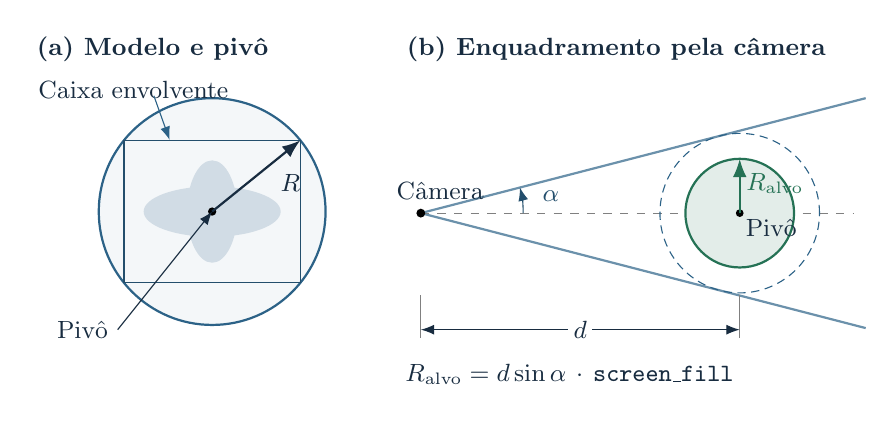
\begin{tikzpicture}[x=1cm,y=1cm,>=Latex,draw=ink,text=ink,font=\small]
\node[anchor=west,font=\small\bfseries] at (0,2.7) {(a) Modelo e pivô};
\coordinate (P) at (2.35,0.64);
\draw[blue,thick,fill=blue!5] (P) circle (1.44);
\draw[blue!80!black] (1.23,-0.265) rectangle (3.47,1.545);
\fill[blue!22] (2.35,0.64) ellipse (0.87 and 0.32);
\fill[blue!22] (2.35,0.64) ellipse (0.32 and 0.65);
\fill (P) circle (1.5pt);
\draw[->,thick] (P) -- (3.47,1.545) node[pos=.66,below right] {$R$};
\draw[<-] (P) -- (1.15,-.86) node[anchor=east] {Pivô};
\node[anchor=west] at (0.02,2.19) {Caixa envolvente};
\draw[->,blue] (1.61,2.11) -- (1.81,1.55);
\node[anchor=west,font=\small\bfseries] at (4.7,2.7) {(b) Enquadramento pela câmera};
\coordinate (C) at (5.0,.62);
\coordinate (O) at (9.05,.62);
\coordinate (U) at (10.65,2.08);
\coordinate (L) at (10.65,-.84);
\draw[blue!70,thick] (U) -- (C) -- (L);
\draw[gray,dashed] (C) -- (10.5,.62);
\pic[draw,blue!80!black,->,"$\alpha$",angle radius=13mm,angle eccentricity=1.28] {angle=O--C--U};
\pgfmathsetmacro{\radlim}{4.05*sin(atan(1.46/5.65))}
\draw[blue,densely dashed] (O) circle (\radlim);
\draw[green,thick,fill=green!13] (O) circle (.69);
\fill (C) circle (1.6pt);
\node[anchor=south west] at (4.57,.67) {Câmera};
\fill (O) circle (1.4pt) node[below right,inner sep=2pt] {Pivô};
\draw[green,->,thick] (O) -- ++(0,.69) node[pos=.54,right,inner sep=2pt] {$R_{\mathrm{alvo}}$};
\draw[thin,gray] (5,-.42) -- (5,-.96) (9.05,-.42) -- (9.05,-.96);
\draw[<->] (5,-.86) -- (9.05,-.86) node[midway,fill=white,inner sep=2pt] {$d$};
\node[anchor=west,align=left] at (4.68,-1.43) {$R_{\mathrm{alvo}}=d\sin\alpha\,\cdot\,\texttt{screen\_fill}$};
\end{tikzpicture}
\end{document}
